\section{Експериментальне дослідження моделі}
\label{sec:experiment}

\subsection{Мета експериментального дослідження}

Мета дослідження задана умовою: знайти кількість посадкових смуг $n$, за якої час окупності додаткових смуг $T$ мінімальний. Отже, модель використовується для оптимізації з одним фактором -- кількістю смуг $n = 2 + k$, де $k = 0, \ldots, 10$ -- і відгуком $T$, обчисленим за формулою \eqref{eq:payback}. Фактор дискретний і має лише 11~значень, тому оптимум шукається повним перебором усіх значень~\cite{stetsenko2024}.

Час окупності обчислюється з річного прибутку $P$, тому умови одного експерименту (тривалість прогону, розгін, кількість повторних прогонів) визначено саме для $P$. Прибуток є відгуком, що стабілізується з часом: це середня швидкість накопичення грошей, на відміну, наприклад, від кількості посадок, що зростає разом із часом моделювання.

Корисно оцінити завантаження смуг: літаки займають у середньому $\lambda \cdot t_s = 35/6 \approx 5{,}83$~смуги. Отже, за $n \le 5$ смуги перевантажені, черга обмежена лише тим, що літаки відлітають після 140~хв, а за $n \ge 6$ смуг вистачає для всього потоку, і черга стає короткою. Цим пояснюється різкий перелом у результатах між $n = 5$ і $n = 7$.

\subsection{Перехідний період і тривалість прогону}

На початку прогону аеропорт порожній: черги немає, і перші літаки сідають без очікування. Такий стан нетиповий для двох смуг, де в сталому режимі черга тримається близько 23~літаків. Щоб визначити тривалість перехідного періоду й тривалість прогону, проведено 4~пробні прогони на 120~діб для $n = 2$ і $n = 7$ і на кожну добу $t$ обчислено оцінку річного прибутку за інтервалом $[0; t]$. Тривалість прогону $T_{\text{mod}}$ визначається умовою~\cite{stetsenko2024}
\begin{equation}
T_{\text{mod}}: \ \forall i, j \quad |y_i(T_{\text{mod}}) - y_j(T_{\text{mod}})| < \varepsilon,
\label{eq:transient}
\end{equation}
де $y_i(t)$ -- оцінка відгуку в $i$-му прогоні за інтервалом $[0; t]$, $\varepsilon$ -- задана точність. Тут $\varepsilon$ узято рівним 2~\% середнього значення оцінки.

Результати наведено на рисунках~\ref{fig:transient-2} і~\ref{fig:transient-7}. За $n = 2$ оцінки чотирьох прогонів відрізняються менше ніж на 2~\% від 91-ї доби, за $n = 7$ -- від 28-ї доби. Тривалість прогону прийнято з запасом рівною одному року модельного часу (525\,600~хв). Рік ще й зручний тим, що прибуток за прогін і є річним прибутком $p$ з формули окупності.

\begin{figure}[H]
\centering
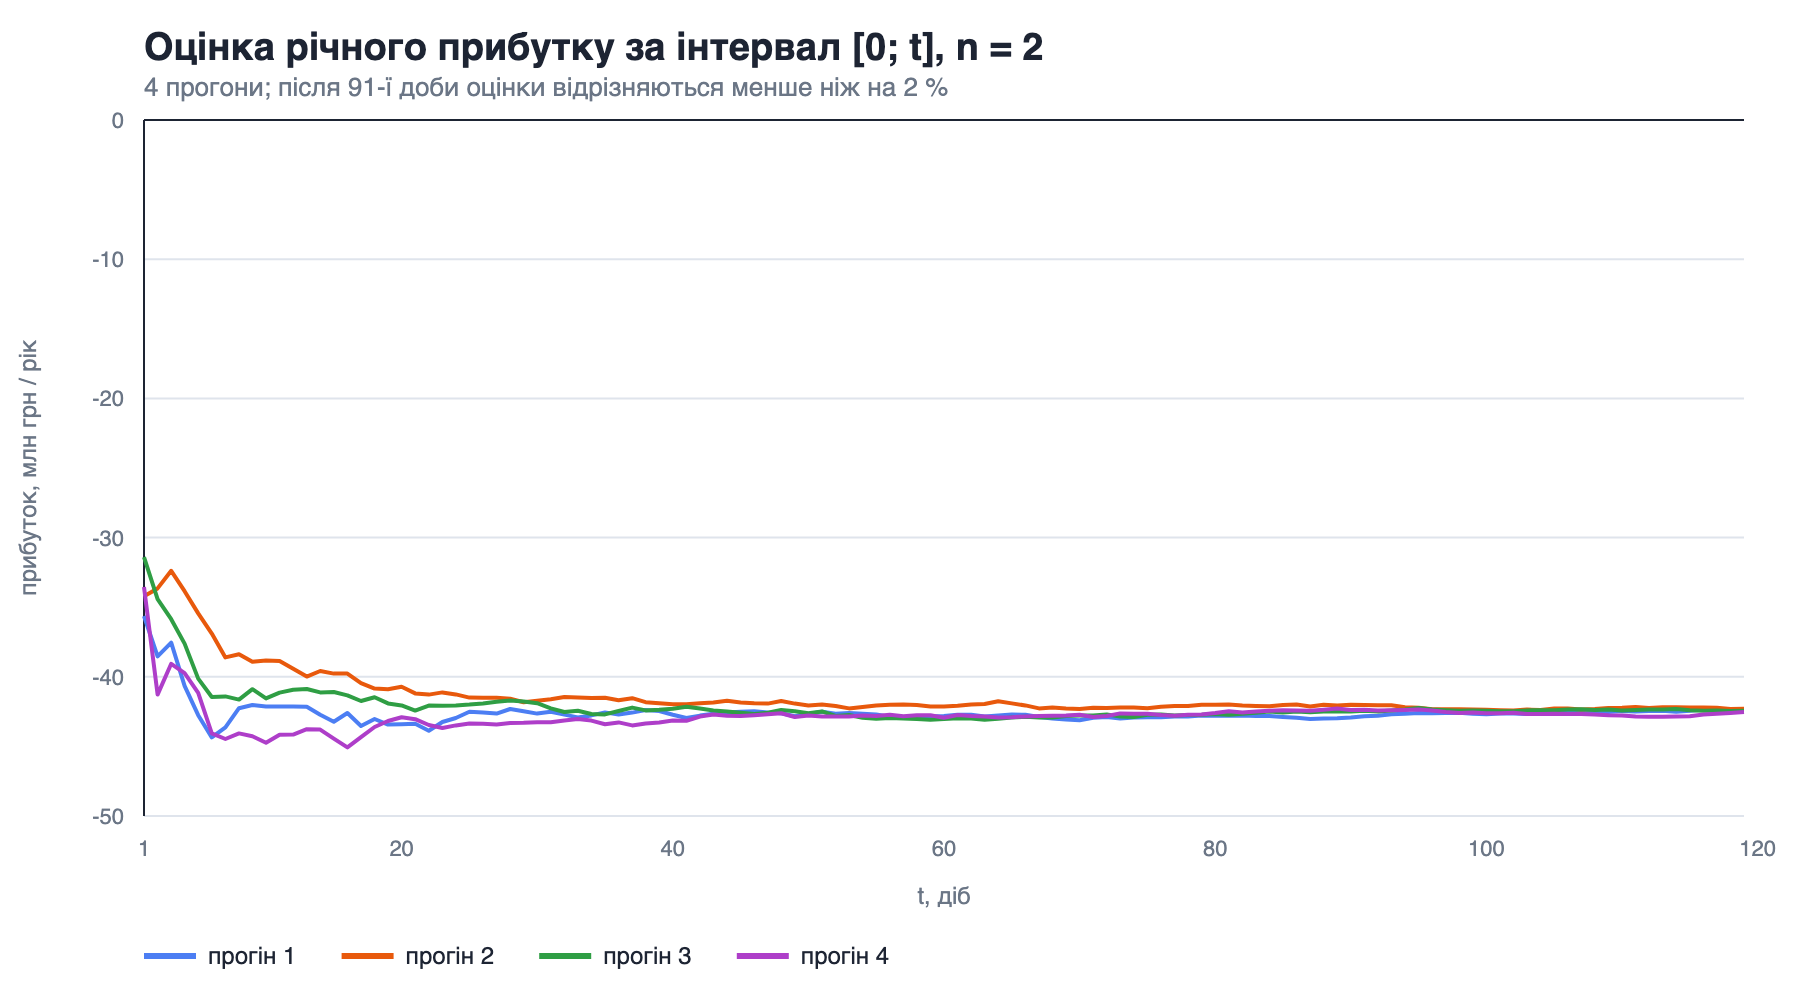
\includegraphics[width=0.92\textwidth]{transient-2.png}
\caption{Оцінка річного прибутку за інтервал $[0; t]$ у чотирьох прогонах, $n = 2$}
\label{fig:transient-2}
\end{figure}

\begin{figure}[H]
\centering
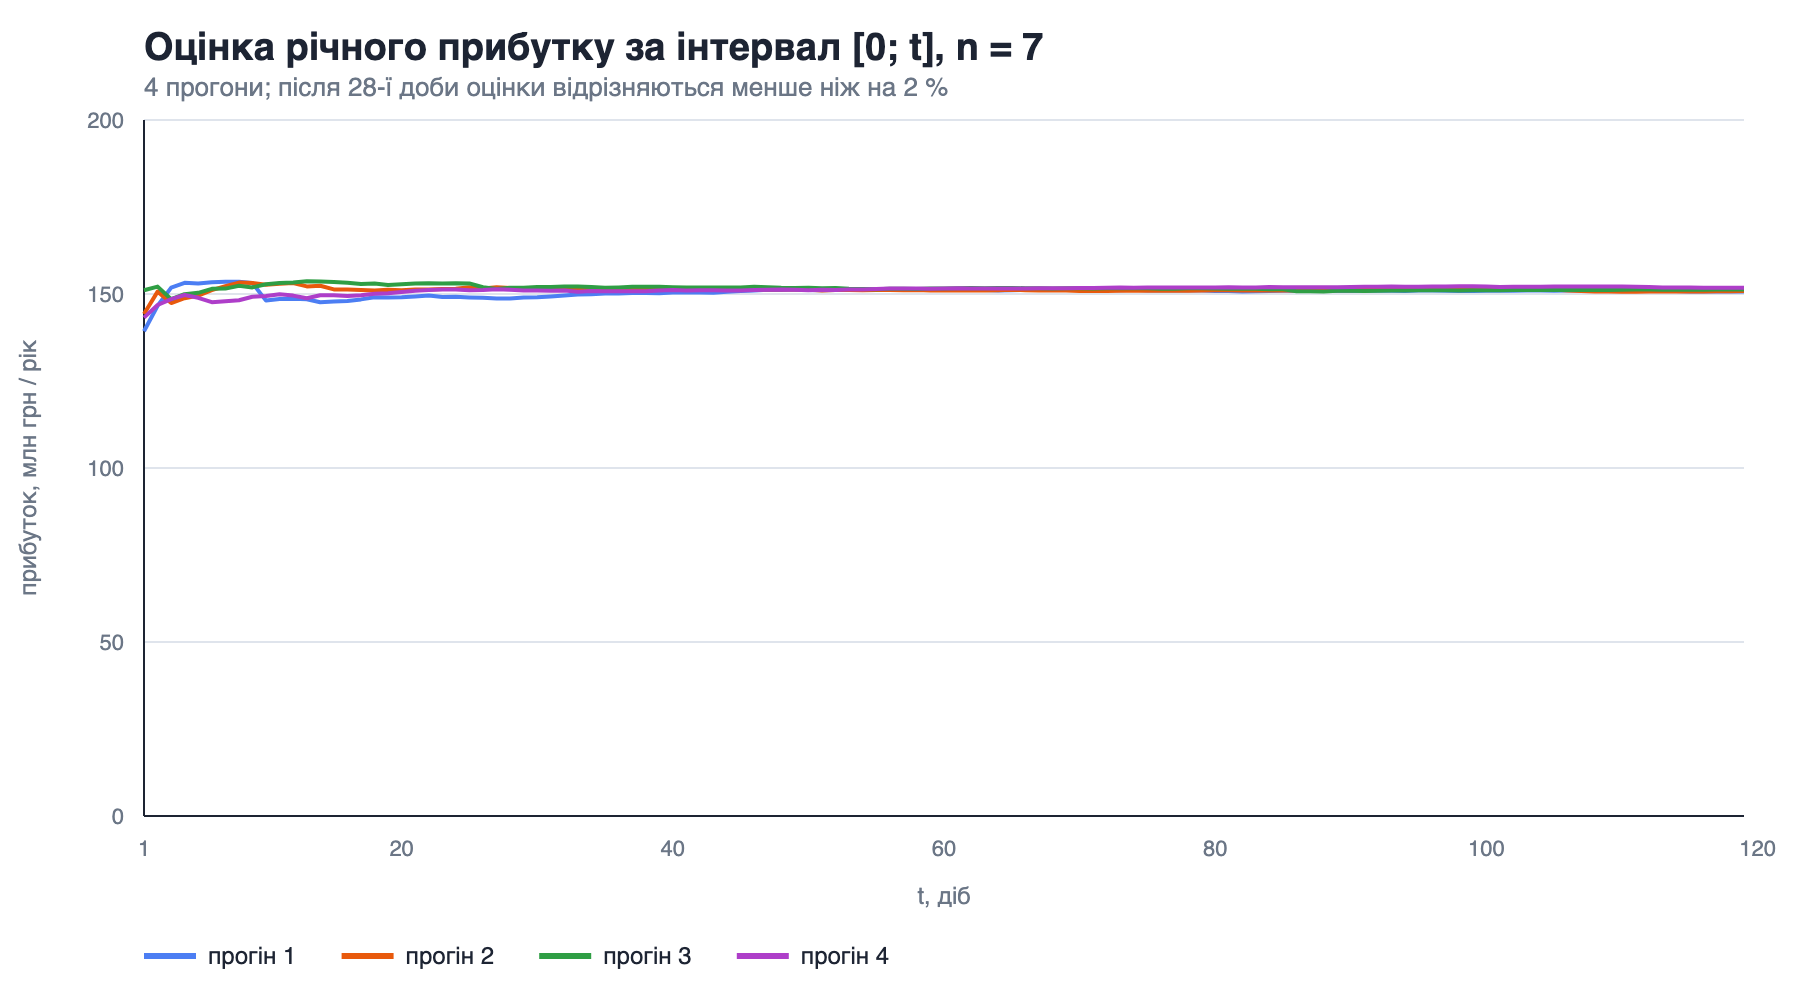
\includegraphics[width=0.92\textwidth]{transient-7.png}
\caption{Оцінка річного прибутку за інтервал $[0; t]$ у чотирьох прогонах, $n = 7$}
\label{fig:transient-7}
\end{figure}

Сам перехідний період значно коротший. На рисунку~\ref{fig:transient-hourly} показано прибуток за кожну годину перших двох діб, усереднений за чотирма прогонами. Нетиповими є лише перші 2--3~години: черга ще не накопичилась, дозаправок немає, і прибуток за годину завищений. Щоб ці години не впливали на результат, статистика збирається після розгону тривалістю одна доба (1440~хв). Отже, кожен прогін триває $T_w + T_m = 1440 + 525\,600 = 527\,040$~хв.

\begin{figure}[H]
\centering
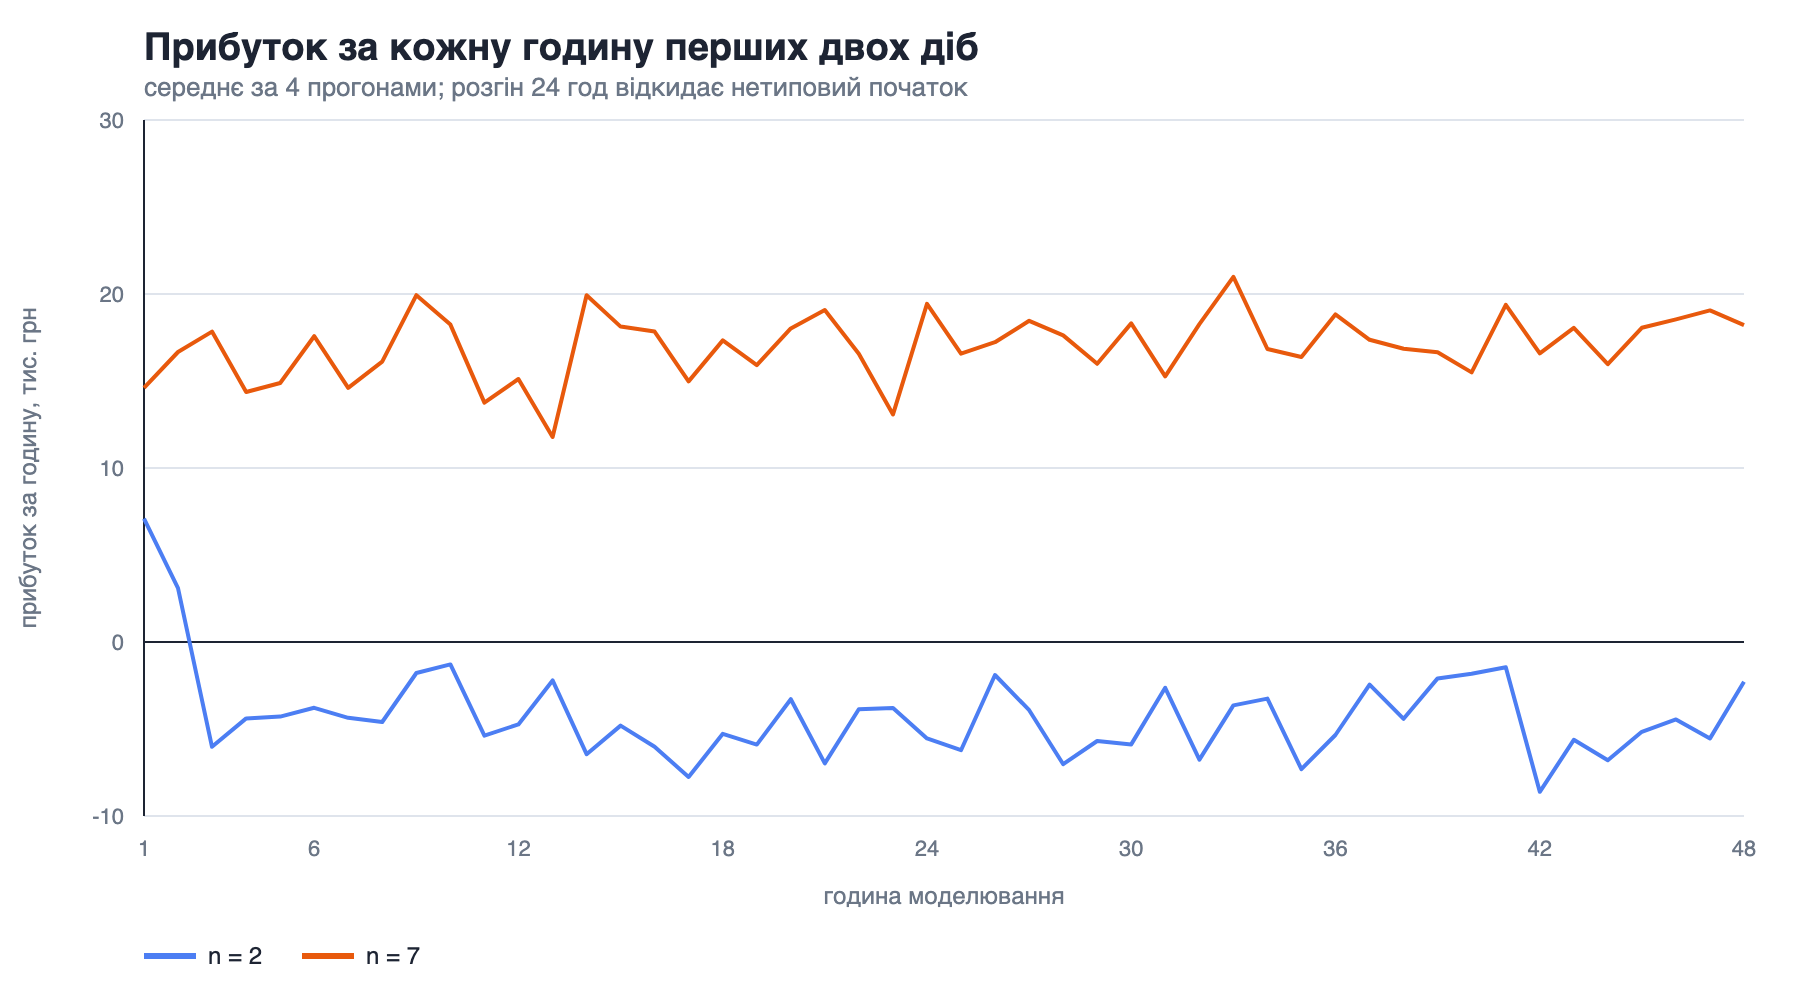
\includegraphics[width=0.92\textwidth]{transient-hourly.png}
\caption{Прибуток аеропорту за кожну годину перших двох діб}
\label{fig:transient-hourly}
\end{figure}

\subsection{Кількість повторних прогонів}

Кількість прогонів, що забезпечує точність $\varepsilon$ з довірчою ймовірністю $\beta = 0{,}95$, визначається наслідком нерівності Чебишева~\cite{stetsenko2024}:
\begin{equation}
p = \frac{\sigma^2}{\varepsilon^2 (1 - \beta)} = 20 \cdot \frac{\sigma^2}{\varepsilon^2},
\label{eq:runs}
\end{equation}
де $\sigma$ -- стандартне відхилення річного прибутку між прогонами, оцінене за 10~пробними прогонами для кожної кількості смуг.

Точність задано в абсолютних одиницях: $\varepsilon = 1$~млн~грн/рік. Відносна точність тут непридатна, бо за чотирьох смуг прибуток близький до нуля (2,6~млн~грн/рік), і 2~\% від нього вимагали б тисяч прогонів. Похибка в 1~млн~грн/рік відповідає менш ніж 1~\% прибутку за $n \ge 6$ і в рази менша за різницю прибутків між сусідніми значеннями $n$ (таблиця~\ref{tab:payback}), тож вона не може змінити вибір оптимуму.

\begin{kpitable}{|L{3.0cm}|L{4.4cm}|L{4.4cm}|L{3.6cm}|}{Кількість прогонів для точності 1~млн~грн/рік\label{tab:runs}}{\textbf{Кількість смуг $n$} & \textbf{Середній прибуток, млн грн/рік} & \textbf{$\sigma$, млн грн/рік} & \textbf{Потрібно прогонів $p$}}
2 & \textminus{}42,476 & 0,259 & 2 \\ \hline
3 & \textminus{}19,941 & 0,216 & 1 \\ \hline
4 & 2,615 & 0,244 & 2 \\ \hline
5 & 28,703 & 0,527 & 6 \\ \hline
6 & 108,146 & 1,587 & 51 \\ \hline
7 & 151,229 & 0,235 & 2 \\ \hline
8 & 162,273 & 0,243 & 2 \\ \hline
9 & 168,386 & 0,293 & 2 \\ \hline
10 & 171,700 & 0,508 & 6 \\ \hline
11 & 173,567 & 0,390 & 4 \\ \hline
12 & 174,477 & 0,606 & 8 \\ \hline

\end{kpitable}

Результати наведено в таблиці~\ref{tab:runs}. Найбільший розкид має $n = 6$: за цієї кількості смуг їх завантаження близьке до одиниці (5,83 з 6), і черга то накопичується, то розсмоктується, тож прибуток окремого року сильно залежить від випадку. Для неї потрібен 51~прогін; цю кількість прийнято для всіх значень $n$, щоб точність була не гіршою за задану для кожного з них.

\subsection{Метод і послідовність експериментів}

Для кожного $k = 0, \ldots, 10$ проведено 51~прогін моделі з $n = 2 + k$ смугами, тривалістю 527\,040~хв кожен, зі збором статистики після першої доби. Загалом це 561~прогін, або 561~рік модельного часу.

Прогони з однаковим номером $i$ для всіх $n$ використовують однакове початкове значення генератора (метод спільних випадкових чисел~\cite{law2015}). Аеропорти з різною кількістю смуг тоді отримують однаковий потік літаків, і різниця прибутків $P(n) - P(2)$ залежить від кількості смуг, а не від того, що одному з варіантів випало більше літаків. Тому час окупності $T_{\Delta}$ обчислюється в кожному прогоні окремо, з прибутків тієї самої пари прогонів, а результатом є середнє за 51~значенням і половина ширини 95~\% довірчого інтервалу за розподілом Стьюдента.

Експерименти проводить функція \code{payback} модуля \code{experiments.ts}:
\begin{Verbatim}
const samples = Array.from({ length: MAX_EXTRA_RUNWAYS + 1 }, (_, extra) =>
  Array.from({ length: runs }, (_, i) =>
    run({ ...params, runways: params.runways + extra }, seed + i)),
);
const base = samples[0] ?? [];
return samples.map((rs, extra) => {
  const cost = extra * params.runwayCost;
  const gains = rs.map((r, i) => r.yearProfit - (base[i]?.yearProfit ?? 0));
  ...
  paybackGain: extra ? estimate(gains.map((g) => cost / g)) : undefined,
\end{Verbatim}
Повний код експериментів наведено в додатку~\ref{app:experiments}. Усі експерименти разом із побудовою графіків запускає команда \code{bun run start}.

\subsection{Результати експериментів}

Середні значення вихідних характеристик за 51~прогоном наведено в таблиці~\ref{tab:payback}. Кількості літаків наведено за рік модельного часу.

\begingroup
\fontsize{12}{14}\selectfont
\begin{kpitable}{|L{0.6cm}|L{1.7cm}|L{1.6cm}|L{1.3cm}|L{1.3cm}|L{1.3cm}|L{1.0cm}|L{1.0cm}|L{2.7cm}|L{1.4cm}|}{Результати перебору кількості смуг (51~прогін по 365~діб)\label{tab:payback}}{\textbf{$n$} & \textbf{$P$, млн грн/рік} & \textbf{$\Delta P$, млн грн/рік} & \textbf{$N_a$} & \textbf{$N_l$} & \textbf{$N_r$} & \textbf{$W$, хв} & \textbf{$B$} & \textbf{$T_{\Delta}$, міс.} & \textbf{$T_P$, міс.}}
2 & \textminus{}42,50 & 0,00 & 87547 & 57511 & 87544 & 132,1 & 2,000 & -- & -- \\ \hline
3 & \textminus{}20,01 & 22,49 & 87615 & 42564 & 87597 & 130,0 & 3,000 & 1,601 $\pm$ 0,007 & -- \\ \hline
4 & 2,63 & 45,12 & 87641 & 27574 & 87479 & 126,9 & 4,000 & 1,596 $\pm$ 0,004 & 27,809 \\ \hline
5 & 28,59 & 71,09 & 87589 & 12519 & 84041 & 116,5 & 4,999 & 1,519 $\pm$ 0,004 & 3,779 \\ \hline
6 & 107,68 & 150,17 & 87526 & 786 & 27218 & 49,4 & 5,776 & 0,959 $\pm$ 0,004 & 1,338 \\ \hline
7 & 151,24 & 193,74 & 87607 & 0 & 479 & 8,8 & 5,834 & 0,929 $\pm$ 0,001 & 1,190 \\ \hline
8 & 162,18 & 204,68 & 87647 & 0 & 6 & 2,9 & 5,836 & 1,055 $\pm$ 0,001 & 1,332 \\ \hline
9 & 168,27 & 210,76 & 87572 & 0 & 0 & 1,1 & 5,831 & 1,196 $\pm$ 0,001 & 1,498 \\ \hline
10 & 171,70 & 214,20 & 87599 & 0 & 0 & 0,4 & 5,833 & 1,345 $\pm$ 0,001 & 1,677 \\ \hline
11 & 173,50 & 216,00 & 87576 & 0 & 0 & 0,2 & 5,832 & 1,500 $\pm$ 0,001 & 1,867 \\ \hline
12 & 174,46 & 216,96 & 87601 & 0 & 0 & 0,1 & 5,833 & 1,659 $\pm$ 0,001 & 2,064 \\ \hline

\end{kpitable}
\endgroup

Залежність прибутку від кількості смуг показано на рисунку~\ref{fig:profit}. За двох смуг аеропорт збитковий: $-42{,}5$~млн~грн/рік. Причина видно з таблиці~\ref{tab:payback}: майже кожен літак, що прибув, стає в чергу і дозаправляється (87\,544 дозаправки на 87\,547 літаків), а сідають лише ті близько 30\,000 літаків на рік, яких можуть прийняти дві смуги ($2 \cdot 525\,600 / 35 \approx 30\,034$); решта 57\,511 відлітають. Витрати на дозаправку всіх літаків перевищують дохід від тих, що сіли. З кожною новою смугою прибуток зростає, найшвидше -- між $n = 5$ і $n = 7$, коли смуг стає достатньо для всього потоку. Після $n = 7$ відльотів уже немає, і кожна наступна смуга лише трохи скорочує очікування, тому приріст прибутку швидко зменшується.

\begin{figure}[H]
\centering
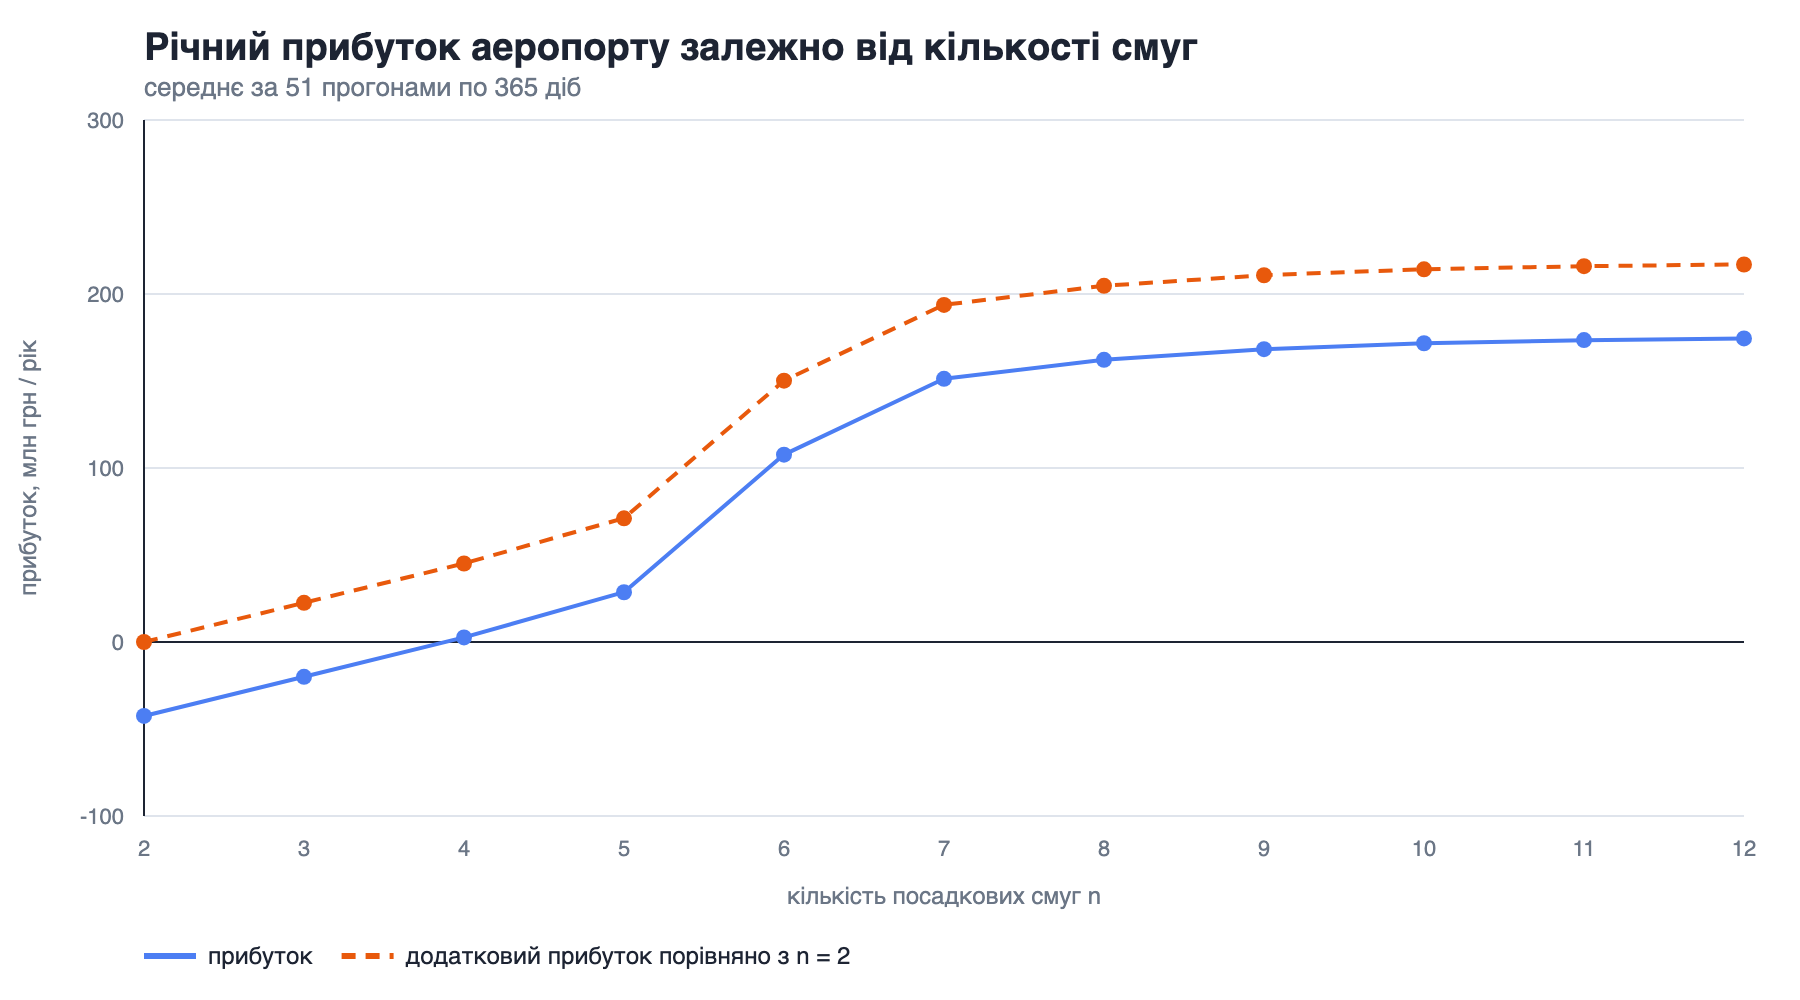
\includegraphics[width=0.92\textwidth]{profit.png}
\caption{Річний прибуток аеропорту залежно від кількості смуг}
\label{fig:profit}
\end{figure}

Як змінюється доля літаків, показано на рисунку~\ref{fig:outcomes}. Частка літаків, що відлітають, падає з 66~\% за двох смуг до нуля за семи; частка дозаправлених -- зі 100~\% до 0,5~\%.

\begin{figure}[H]
\centering
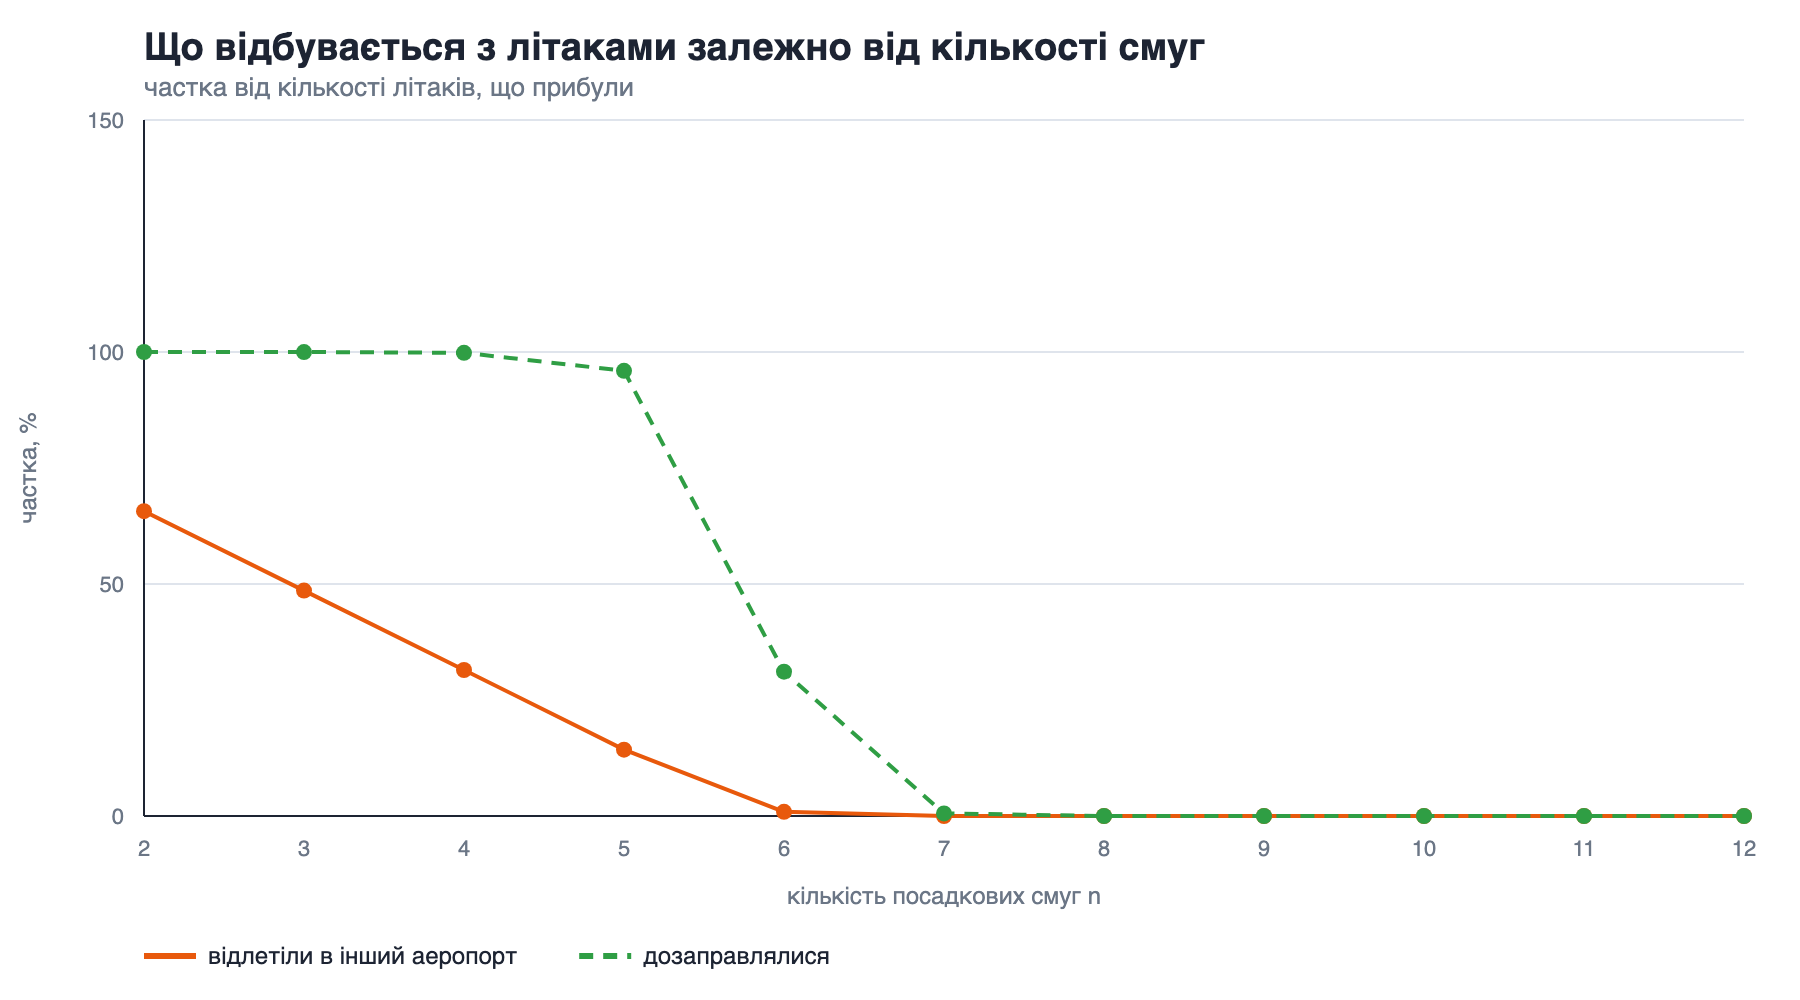
\includegraphics[width=0.92\textwidth]{outcomes.png}
\caption{Частки літаків, що відлетіли й дозаправлялися, залежно від кількості смуг}
\label{fig:outcomes}
\end{figure}

Час окупності показано на рисунку~\ref{fig:payback}. Витрати на смуги зростають лінійно, а приріст прибутку -- спершу швидко, потім дедалі повільніше, тому $T$ має мінімум. За обома інтерпретаціями прибутку $p$ мінімум досягається за $n = 7$: $T_{\Delta} = 0{,}929$~міс. і $T_P = 1{,}190$~міс. Найближчі сусіди, $n = 6$ і $n = 8$, дають $T_{\Delta} = 0{,}959$ і 1,055~міс. Половина ширини довірчого інтервалу для $T_{\Delta}$ не перевищує 0,007~міс. (таблиця~\ref{tab:payback}), тобто довірчі інтервали сусідніх варіантів не перетинаються, і оптимум визначено надійно.

\begin{figure}[H]
\centering
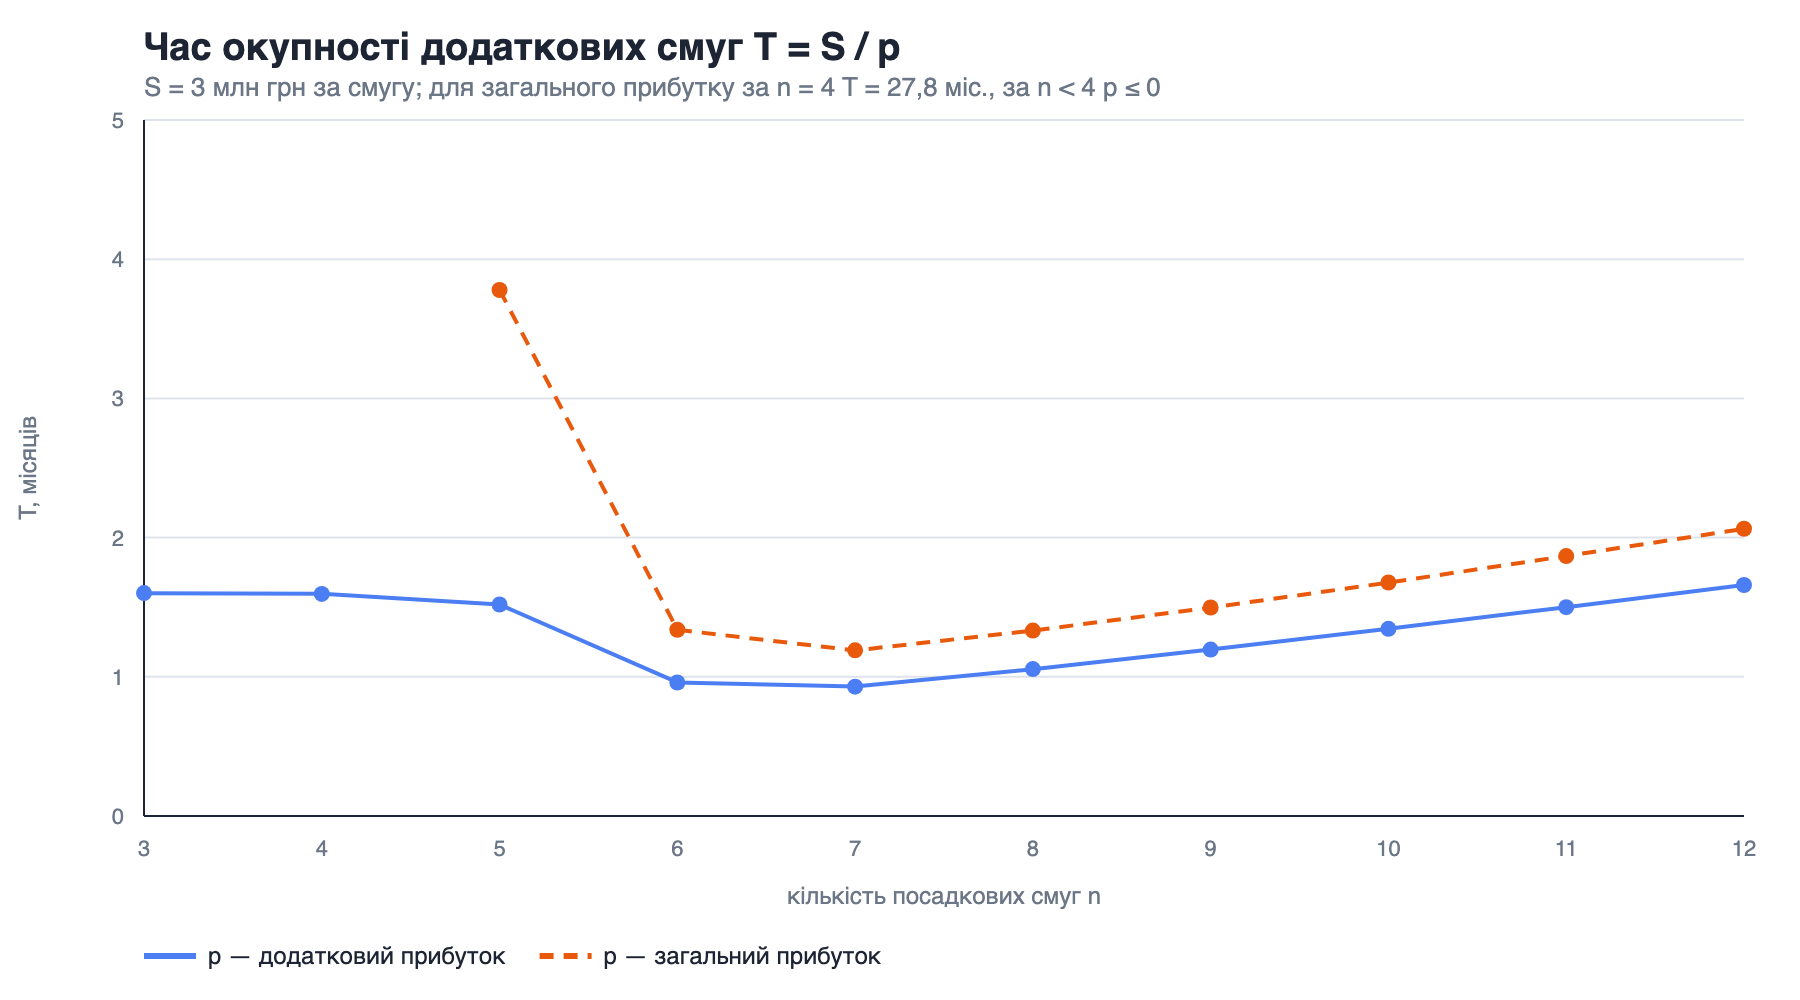
\includegraphics[width=0.92\textwidth]{payback.png}
\caption{Час окупності додаткових смуг залежно від кількості смуг}
\label{fig:payback}
\end{figure}

\subsection{Висновки до розділу}

Визначено умови одного експерименту: прогін тривалістю рік модельного часу після розгону на одну добу, що відкидає нетиповий початок. Для точності 1~млн~грн/рік з довірчою ймовірністю 0,95 потрібен 51~прогін. Повним перебором 11~варіантів з методом спільних випадкових чисел встановлено, що час окупності мінімальний за семи смуг, тобто за п'яти додаткових: 0,929~міс. за приростом прибутку і 1,190~міс. за загальним прибутком.
